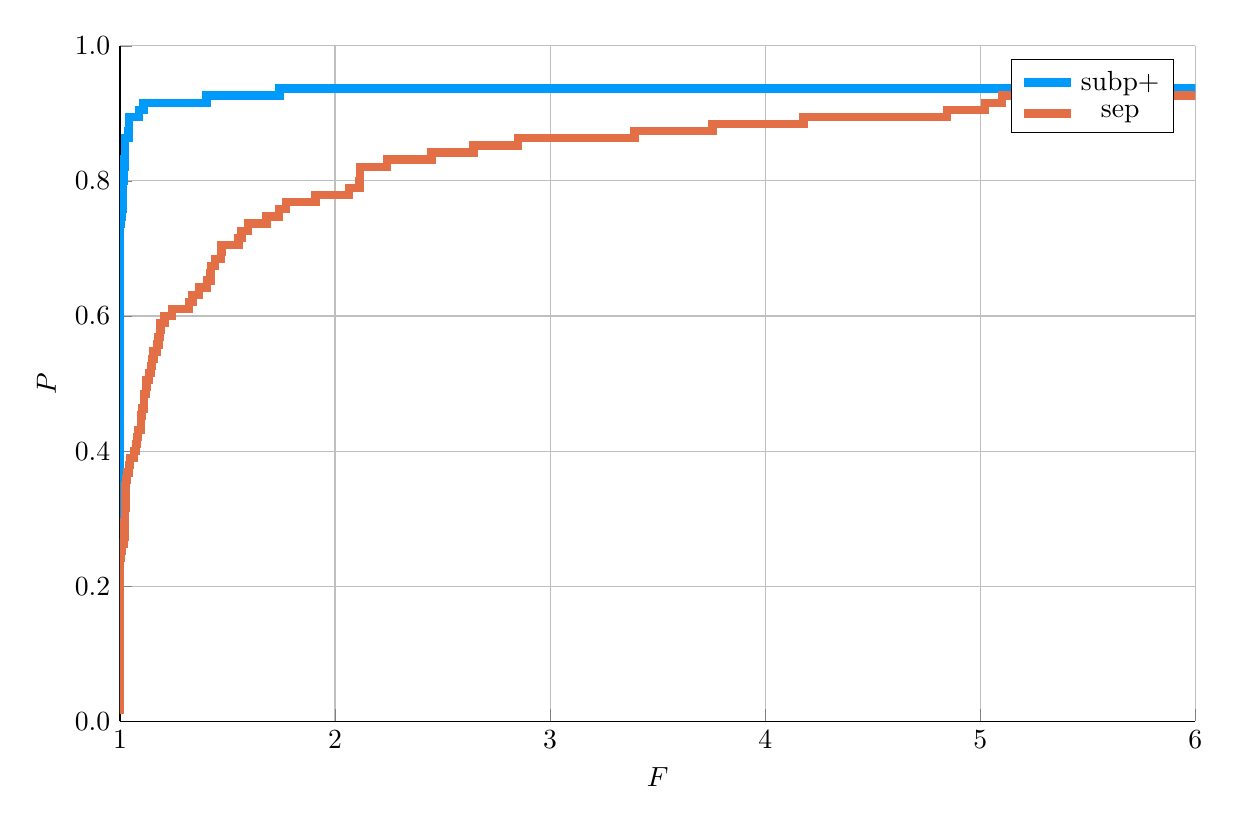
\begin{tikzpicture}[]
\begin{axis}[height = {101.6mm}, ylabel = {$P$}, xmin = {1.0}, xmax = {6}, ymax = {1.0}, xlabel = {$F$}, {unbounded coords=jump, xticklabel style={rotate = 0}, xmajorgrids = true, xtick = {1.0,2.0,3.0,4.0,5.0,6.0}, xticklabels = {1,2,3,4,5,6}, xtick align = inside, axis lines* = left, yticklabel style={rotate = 0}, ymajorgrids = true, ytick = {0.0,0.2,0.4,0.6000000000000001,0.8,1.0}, yticklabels = {0.0,0.2,0.4,0.6,0.8,1.0}, ytick align = inside, axis lines* = left,     xshift = 0.0mm,
    yshift = 0.0mm,
    axis background/.style={fill={rgb,1:red,1.00000000;green,1.00000000;blue,1.00000000}}
}, ymin = {0}, width = {152.4mm}]\addplot+ [color = {rgb,1:red,0.00000000;green,0.60560316;blue,0.97868012},
draw opacity=1.0,
line width=3,
solid,mark = none,
mark size = 2.0,
mark options = {
    color = {rgb,1:red,0.00000000;green,0.00000000;blue,0.00000000}, draw opacity = 1.0,
    fill = {rgb,1:red,0.00000000;green,0.60560316;blue,0.97868012}, fill opacity = 1.0,
    line width = 1,
    rotate = 0,
    solid
},const plot]coordinates {
(1.0, 0.010526315789473684)
(1.0, 0.021052631578947368)
(1.0, 0.031578947368421054)
(1.0, 0.042105263157894736)
(1.0, 0.05263157894736842)
(1.0, 0.06315789473684211)
(1.0, 0.07368421052631578)
(1.0, 0.08421052631578947)
(1.0, 0.09473684210526316)
(1.0, 0.10526315789473684)
(1.0, 0.11578947368421053)
(1.0, 0.12631578947368421)
(1.0, 0.1368421052631579)
(1.0, 0.14736842105263157)
(1.0, 0.15789473684210525)
(1.0, 0.16842105263157894)
(1.0, 0.17894736842105263)
(1.0, 0.18947368421052632)
(1.0, 0.2)
(1.0, 0.21052631578947367)
(1.0, 0.22105263157894736)
(1.0, 0.23157894736842105)
(1.0, 0.24210526315789474)
(1.0, 0.25263157894736843)
(1.0, 0.2631578947368421)
(1.0, 0.2736842105263158)
(1.0, 0.28421052631578947)
(1.0, 0.29473684210526313)
(1.0, 0.30526315789473685)
(1.0, 0.3157894736842105)
(1.0, 0.3263157894736842)
(1.0, 0.3368421052631579)
(1.0, 0.3473684210526316)
(1.0, 0.35789473684210527)
(1.0, 0.3684210526315789)
(1.0, 0.37894736842105264)
(1.0, 0.3894736842105263)
(1.0, 0.4)
(1.0, 0.4105263157894737)
(1.0, 0.42105263157894735)
(1.0, 0.43157894736842106)
(1.0, 0.4421052631578947)
(1.0, 0.45263157894736844)
(1.0, 0.4631578947368421)
(1.0, 0.47368421052631576)
(1.0, 0.4842105263157895)
(1.0, 0.49473684210526314)
(1.0, 0.5052631578947369)
(1.0, 0.5157894736842106)
(1.0, 0.5263157894736842)
(1.0, 0.5368421052631579)
(1.0, 0.5473684210526316)
(1.0, 0.5578947368421052)
(1.0, 0.5684210526315789)
(1.0, 0.5789473684210527)
(1.0, 0.5894736842105263)
(1.0, 0.6)
(1.0, 0.6105263157894737)
(1.0, 0.6210526315789474)
(1.0, 0.631578947368421)
(1.0, 0.6421052631578947)
(1.0, 0.6526315789473685)
(1.0, 0.6631578947368421)
(1.0, 0.6736842105263158)
(1.0, 0.6842105263157895)
(1.0, 0.6947368421052632)
(1.0, 0.7052631578947368)
(1.0, 0.7157894736842105)
(1.0, 0.7263157894736842)
(1.0, 0.7368421052631579)
(1.0030975605396197, 0.7473684210526316)
(1.0092210830554056, 0.7578947368421053)
(1.0115029054497995, 0.7684210526315789)
(1.0115334250179806, 0.7789473684210526)
(1.0116477277393388, 0.7894736842105263)
(1.015222835476184, 0.8)
(1.015845742691571, 0.8105263157894737)
(1.018149222463464, 0.8210526315789474)
(1.021078710452067, 0.8315789473684211)
(1.0221110459429845, 0.8421052631578947)
(1.0235694351929532, 0.8526315789473684)
(1.0238603291079056, 0.8631578947368421)
(1.0395197653267139, 0.8736842105263158)
(1.0418597862133512, 0.8842105263157894)
(1.0424967091943944, 0.8947368421052632)
(1.089464630212187, 0.9052631578947369)
(1.11007971670795, 0.9157894736842105)
(1.4021658839574587, 0.9263157894736842)
(1.742440075880329, 0.9368421052631579)
(10.203297175975841, 0.9473684210526315)
(10.203297175975841, 0.9578947368421052)
(10.203297175975841, 0.968421052631579)
(10.203297175975841, 0.9789473684210527)
(10.203297175975841, 0.9894736842105263)
(10.203297175975841, 1.0)
(10.203297175975841, 1.0105263157894737)
};
\addlegendentry{subp+}
\addplot+ [color = {rgb,1:red,0.88887350;green,0.43564919;blue,0.27812294},
draw opacity=1.0,
line width=3,
solid,mark = none,
mark size = 2.0,
mark options = {
    color = {rgb,1:red,0.00000000;green,0.00000000;blue,0.00000000}, draw opacity = 1.0,
    fill = {rgb,1:red,0.88887350;green,0.43564919;blue,0.27812294}, fill opacity = 1.0,
    line width = 1,
    rotate = 0,
    solid
},const plot]coordinates {
(1.0, 0.010526315789473684)
(1.0, 0.021052631578947368)
(1.0, 0.031578947368421054)
(1.0, 0.042105263157894736)
(1.0, 0.05263157894736842)
(1.0, 0.06315789473684211)
(1.0, 0.07368421052631578)
(1.0, 0.08421052631578947)
(1.0, 0.09473684210526316)
(1.0, 0.10526315789473684)
(1.0, 0.11578947368421053)
(1.0, 0.12631578947368421)
(1.0, 0.1368421052631579)
(1.0, 0.14736842105263157)
(1.0, 0.15789473684210525)
(1.0, 0.16842105263157894)
(1.0, 0.17894736842105263)
(1.0, 0.18947368421052632)
(1.0, 0.2)
(1.0, 0.21052631578947367)
(1.0, 0.22105263157894736)
(1.0005652486800505, 0.23157894736842105)
(1.0013927634967987, 0.24210526315789474)
(1.0037839344863573, 0.25263157894736843)
(1.0066720321260212, 0.2631578947368421)
(1.0203804429149494, 0.2736842105263158)
(1.0213556918585698, 0.28421052631578947)
(1.0215376804150926, 0.29473684210526313)
(1.0223780135321356, 0.30526315789473685)
(1.024238909654171, 0.3157894736842105)
(1.0259179645381733, 0.3263157894736842)
(1.0263586011212857, 0.3368421052631579)
(1.0263965177345264, 0.3473684210526316)
(1.028810162939359, 0.35789473684210527)
(1.0322170433386073, 0.3684210526315789)
(1.043658159706651, 0.37894736842105264)
(1.0471098398968401, 0.3894736842105263)
(1.06695420169205, 0.4)
(1.0752410322858987, 0.4105263157894737)
(1.080281643398441, 0.42105263157894735)
(1.082389582799734, 0.43157894736842106)
(1.0969601678380718, 0.4421052631578947)
(1.0986585457408444, 0.45263157894736844)
(1.1028376618768685, 0.4631578947368421)
(1.1102270829288656, 0.47368421052631576)
(1.1105426880331979, 0.4842105263157895)
(1.1201178418324516, 0.49473684210526314)
(1.123930562607537, 0.5052631578947369)
(1.1361994217164977, 0.5157894736842106)
(1.1431586703146448, 0.5263157894736842)
(1.14815726236475, 0.5368421052631579)
(1.1555254524106364, 0.5473684210526316)
(1.1723738539669644, 0.5578947368421052)
(1.17910127774238, 0.5684210526315789)
(1.1871229907623868, 0.5789473684210527)
(1.18916544266322, 0.5894736842105263)
(1.206608257506424, 0.6)
(1.2430935878240827, 0.6105263157894737)
(1.3200962508726781, 0.6210526315789474)
(1.3369251985639214, 0.631578947368421)
(1.3682907421606139, 0.6421052631578947)
(1.4036572555402542, 0.6526315789473685)
(1.4208168954253138, 0.6631578947368421)
(1.422275261073828, 0.6736842105263158)
(1.4432164553090678, 0.6842105263157895)
(1.4684133140104234, 0.6947368421052632)
(1.472193777043176, 0.7052631578947368)
(1.5513470032147119, 0.7157894736842105)
(1.5644493485649502, 0.7263157894736842)
(1.594392059464761, 0.7368421052631579)
(1.680822430539687, 0.7473684210526316)
(1.7400002601795876, 0.7578947368421053)
(1.7727914714399868, 0.7684210526315789)
(1.9097946986692156, 0.7789473684210526)
(2.064528094001428, 0.7894736842105263)
(2.1130532620013884, 0.8)
(2.114647372105767, 0.8105263157894737)
(2.1162316272755652, 0.8210526315789474)
(2.2431577689122544, 0.8315789473684211)
(2.44810243800913, 0.8421052631578947)
(2.6441128737795965, 0.8526315789473684)
(2.849346777010543, 0.8631578947368421)
(3.3927416813719877, 0.8736842105263158)
(3.7554415520379636, 0.8842105263157894)
(4.178359464893345, 0.8947368421052632)
(4.845808467109558, 0.9052631578947369)
(5.022635833205817, 0.9157894736842105)
(5.1016485879879205, 0.9263157894736842)
(10.203297175975841, 0.9368421052631579)
(10.203297175975841, 0.9473684210526315)
(10.203297175975841, 0.9578947368421052)
(10.203297175975841, 0.968421052631579)
(10.203297175975841, 0.9789473684210527)
(10.203297175975841, 0.9894736842105263)
(10.203297175975841, 1.0)
(10.203297175975841, 1.0105263157894737)
};
\addlegendentry{sep}
\end{axis}

\end{tikzpicture}
